\documentclass{article}\usepackage[]{graphicx}\usepackage[]{xcolor}
% maxwidth is the original width if it is less than linewidth
% otherwise use linewidth (to make sure the graphics do not exceed the margin)
\makeatletter
\def\maxwidth{ %
  \ifdim\Gin@nat@width>\linewidth
    \linewidth
  \else
    \Gin@nat@width
  \fi
}
\makeatother

\definecolor{fgcolor}{rgb}{0.345, 0.345, 0.345}
\newcommand{\hlnum}[1]{\textcolor[rgb]{0.686,0.059,0.569}{#1}}%
\newcommand{\hlstr}[1]{\textcolor[rgb]{0.192,0.494,0.8}{#1}}%
\newcommand{\hlcom}[1]{\textcolor[rgb]{0.678,0.584,0.686}{\textit{#1}}}%
\newcommand{\hlopt}[1]{\textcolor[rgb]{0,0,0}{#1}}%
\newcommand{\hlstd}[1]{\textcolor[rgb]{0.345,0.345,0.345}{#1}}%
\newcommand{\hlkwa}[1]{\textcolor[rgb]{0.161,0.373,0.58}{\textbf{#1}}}%
\newcommand{\hlkwb}[1]{\textcolor[rgb]{0.69,0.353,0.396}{#1}}%
\newcommand{\hlkwc}[1]{\textcolor[rgb]{0.333,0.667,0.333}{#1}}%
\newcommand{\hlkwd}[1]{\textcolor[rgb]{0.737,0.353,0.396}{\textbf{#1}}}%
\let\hlipl\hlkwb

\usepackage{framed}
\makeatletter
\newenvironment{kframe}{%
 \def\at@end@of@kframe{}%
 \ifinner\ifhmode%
  \def\at@end@of@kframe{\end{minipage}}%
  \begin{minipage}{\columnwidth}%
 \fi\fi%
 \def\FrameCommand##1{\hskip\@totalleftmargin \hskip-\fboxsep
 \colorbox{shadecolor}{##1}\hskip-\fboxsep
     % There is no \\@totalrightmargin, so:
     \hskip-\linewidth \hskip-\@totalleftmargin \hskip\columnwidth}%
 \MakeFramed {\advance\hsize-\width
   \@totalleftmargin\z@ \linewidth\hsize
   \@setminipage}}%
 {\par\unskip\endMakeFramed%
 \at@end@of@kframe}
\makeatother

\definecolor{shadecolor}{rgb}{.97, .97, .97}
\definecolor{messagecolor}{rgb}{0, 0, 0}
\definecolor{warningcolor}{rgb}{1, 0, 1}
\definecolor{errorcolor}{rgb}{1, 0, 0}
\newenvironment{knitrout}{}{} % an empty environment to be redefined in TeX

\usepackage{alltt}
\usepackage[sc]{mathpazo}
\renewcommand{\sfdefault}{lmss}
\renewcommand{\ttdefault}{lmtt}
\usepackage[T1]{fontenc}
\usepackage{geometry}
\geometry{verbose,tmargin=2.5cm,bmargin=2.5cm,lmargin=2.5cm,rmargin=2.5cm}
\setcounter{secnumdepth}{2}
\setcounter{tocdepth}{2}
\usepackage[unicode=true,pdfusetitle,
 bookmarks=true,bookmarksnumbered=true,bookmarksopen=true,bookmarksopenlevel=2,
 breaklinks=false,pdfborder={0 0 1},backref=false,colorlinks=false]
 {hyperref}
\hypersetup{
 pdfstartview={XYZ null null 1}}

\makeatletter
%%%%%%%%%%%%%%%%%%%%%%%%%%%%%% User specified LaTeX commands.
\renewcommand{\textfraction}{0.05}
\renewcommand{\topfraction}{0.8}
\renewcommand{\bottomfraction}{0.8}
\renewcommand{\floatpagefraction}{0.75}

\makeatother
\IfFileExists{upquote.sty}{\usepackage{upquote}}{}
\begin{document}








The results below are generated from an R script.

\begin{knitrout}
\definecolor{shadecolor}{rgb}{0.969, 0.969, 0.969}\color{fgcolor}\begin{kframe}
\begin{alltt}
\hlcom{# Assignment: ASSIGNMENT 4}
\hlcom{# Name: Quintero Vasquez, Johnatan}
\hlcom{# Date: 2023-07-16}

\hlcom{## Load the ggplot2 package}
\hlkwd{library}\hlstd{(ggplot2)}
\hlkwd{theme_set}\hlstd{(}\hlkwd{theme_minimal}\hlstd{())}

\hlcom{## Set the working directory to the root of your DSC 520 directory}
\hlkwd{setwd}\hlstd{(}\hlstr{"C:/Users/21428899/OneDrive-Bellevue University/Documents/GitHub/dsc520"}\hlstd{)}

\hlcom{## Load the `data/r4ds/heights.csv` to}
\hlstd{heights_df} \hlkwb{<-} \hlkwd{read.csv}\hlstd{(}\hlstr{"data/r4ds/heights.csv"}\hlstd{)}

\hlcom{# https://ggplot2.tidyverse.org/reference/geom_boxplot.html}
\hlcom{## Create boxplots of sex vs. earn and race vs. earn using `geom_point()` and `geom_boxplot()`}
\hlcom{## sex vs. earn}
\hlkwd{ggplot}\hlstd{(heights_df,} \hlkwd{aes}\hlstd{(}\hlkwc{x} \hlstd{= sex,} \hlkwc{y} \hlstd{= earn))} \hlopt{+} \hlkwd{geom_point}\hlstd{()} \hlopt{+} \hlkwd{geom_boxplot}\hlstd{()}
\end{alltt}
\end{kframe}

{\centering 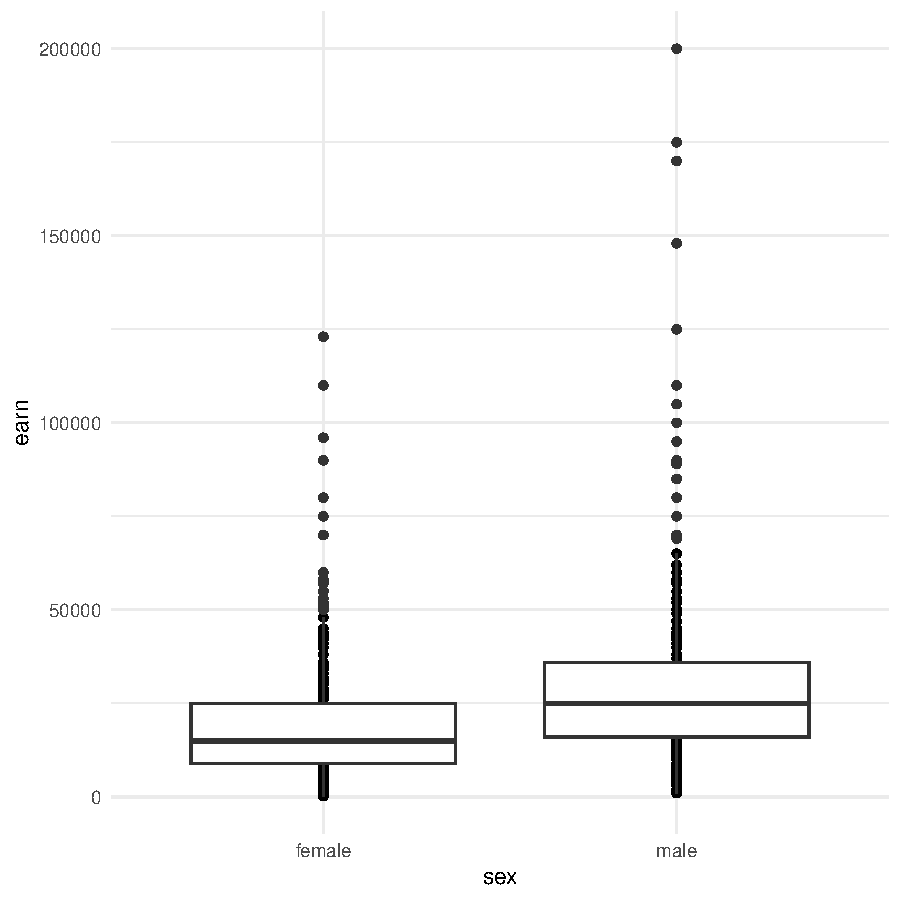
\includegraphics[width=.6\linewidth]{figure/assignment-04-Quintero-Vasquez-Johnatan-Rnwauto-report-1} 

}


\begin{kframe}\begin{alltt}
\hlcom{## race vs. earn}
\hlkwd{ggplot}\hlstd{(heights_df,} \hlkwd{aes}\hlstd{(}\hlkwc{x} \hlstd{= race,} \hlkwc{y} \hlstd{= earn))} \hlopt{+} \hlkwd{geom_point}\hlstd{()} \hlopt{+} \hlkwd{geom_boxplot}\hlstd{()}
\end{alltt}
\end{kframe}

{\centering 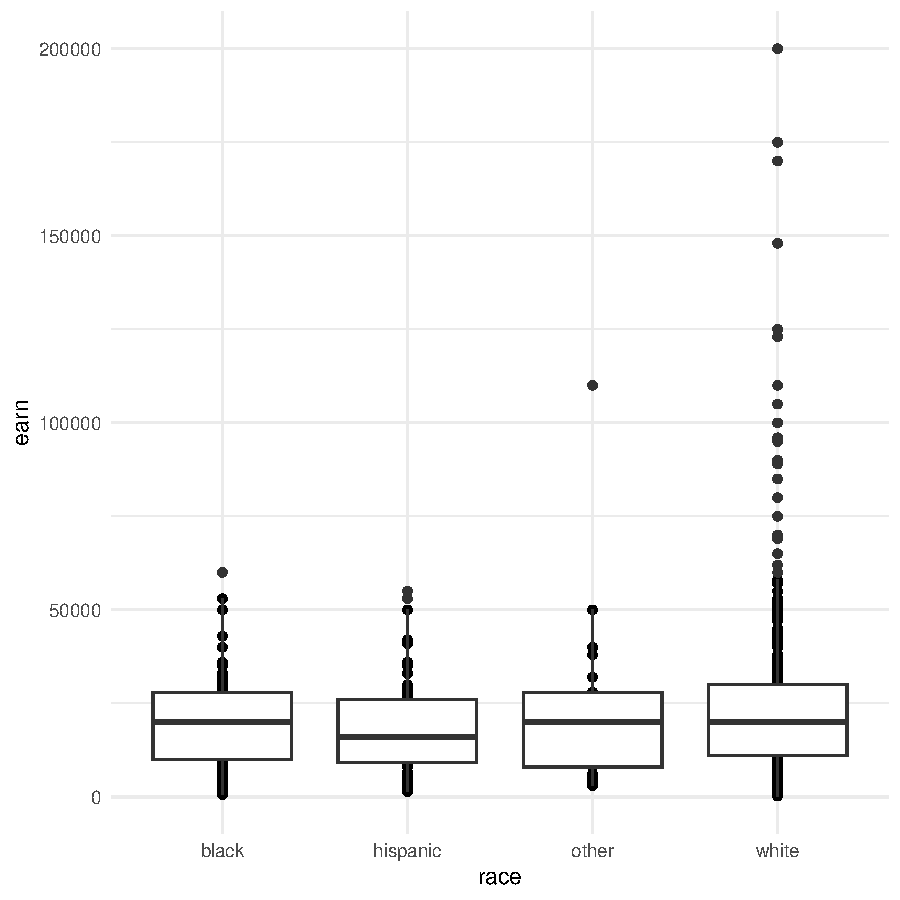
\includegraphics[width=.6\linewidth]{figure/assignment-04-Quintero-Vasquez-Johnatan-Rnwauto-report-2} 

}


\begin{kframe}\begin{alltt}
\hlcom{# https://ggplot2.tidyverse.org/reference/geom_bar.html}
\hlcom{## Using `geom_bar()` plot a bar chart of the number of records for each `sex`}
\hlkwd{ggplot}\hlstd{(heights_df,} \hlkwd{aes}\hlstd{(}\hlkwc{x} \hlstd{= sex))} \hlopt{+} \hlkwd{geom_bar}\hlstd{()}
\end{alltt}
\end{kframe}

{\centering 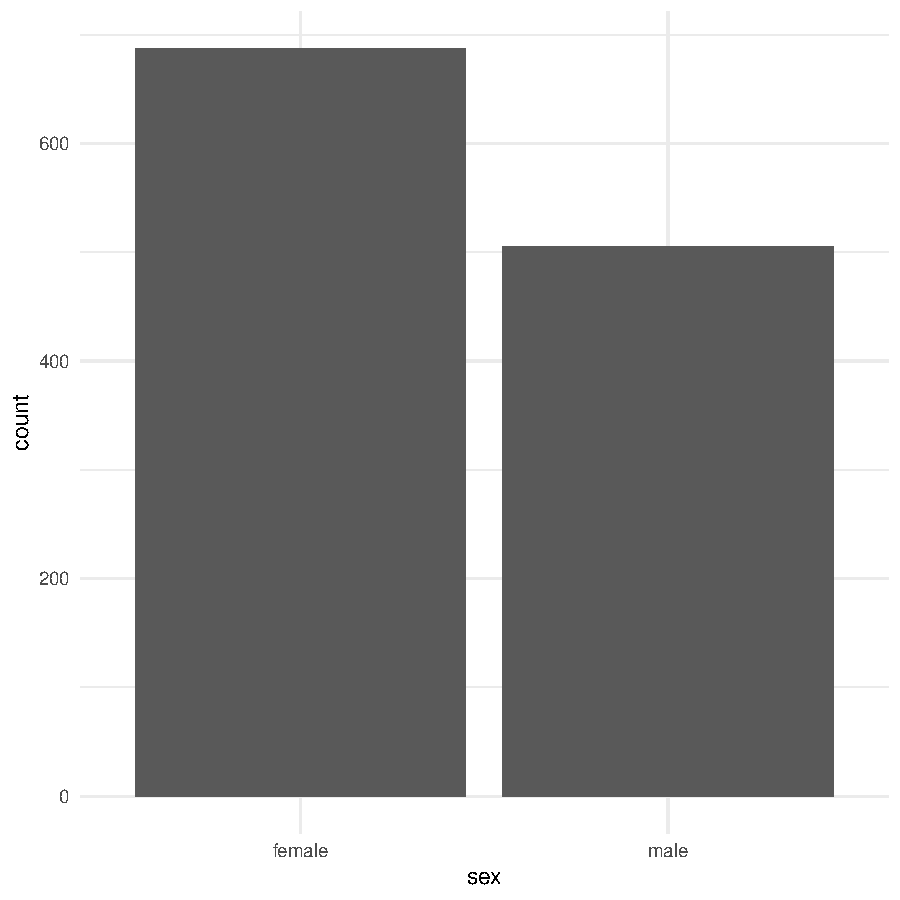
\includegraphics[width=.6\linewidth]{figure/assignment-04-Quintero-Vasquez-Johnatan-Rnwauto-report-3} 

}


\begin{kframe}\begin{alltt}
\hlcom{## Using `geom_bar()` plot a bar chart of the number of records for each race}
\hlkwd{ggplot}\hlstd{(heights_df,} \hlkwd{aes}\hlstd{(}\hlkwc{x} \hlstd{= race))} \hlopt{+} \hlkwd{geom_bar}\hlstd{()}
\end{alltt}
\end{kframe}

{\centering 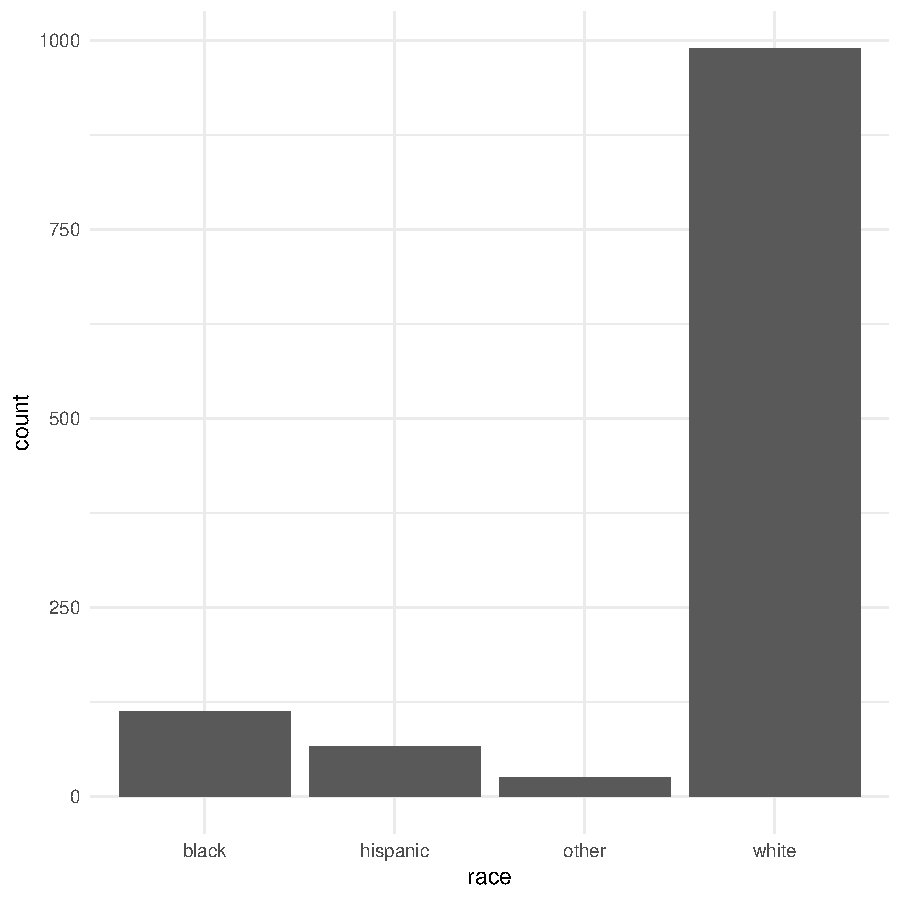
\includegraphics[width=.6\linewidth]{figure/assignment-04-Quintero-Vasquez-Johnatan-Rnwauto-report-4} 

}


\begin{kframe}\begin{alltt}
\hlcom{## Create a horizontal bar chart by adding `coord_flip()` to the previous plot}
\hlkwd{ggplot}\hlstd{(heights_df,} \hlkwd{aes}\hlstd{(}\hlkwc{x} \hlstd{= race))} \hlopt{+} \hlkwd{geom_bar}\hlstd{()} \hlopt{+} \hlkwd{coord_flip}\hlstd{()}
\end{alltt}
\end{kframe}

{\centering 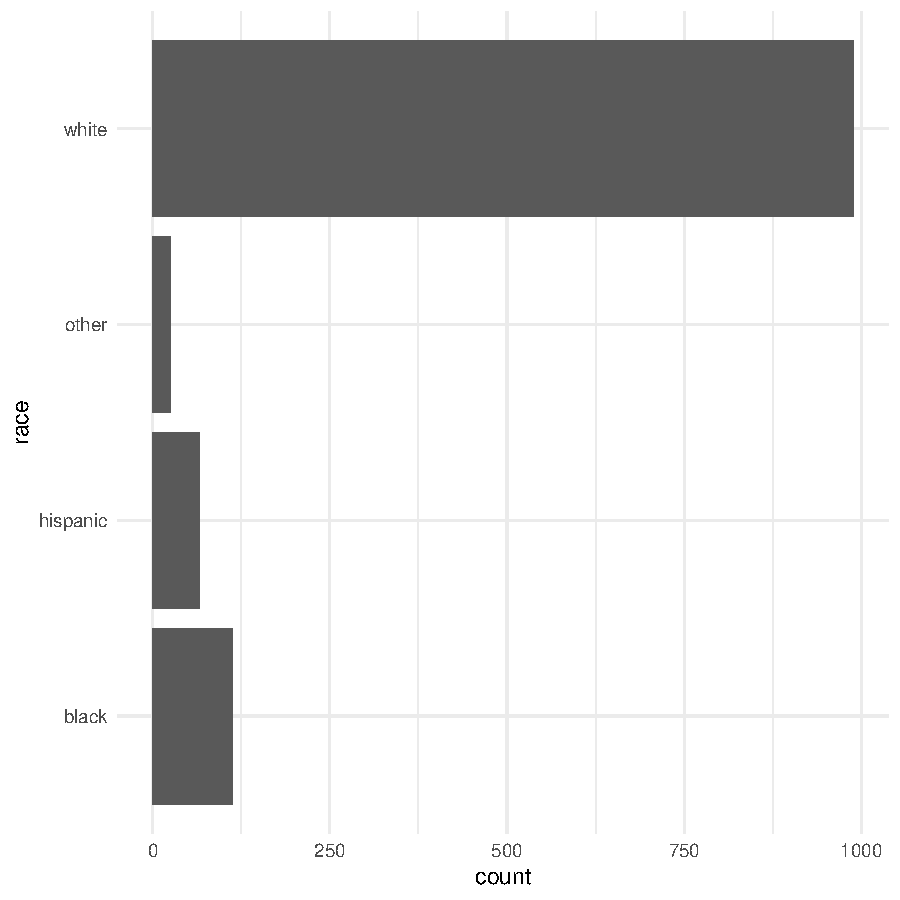
\includegraphics[width=.6\linewidth]{figure/assignment-04-Quintero-Vasquez-Johnatan-Rnwauto-report-5} 

}


\begin{kframe}\begin{alltt}
\hlcom{# https://www.rdocumentation.org/packages/ggplot2/versions/3.3.0/topics/geom_path}
\hlcom{## Load the file `"data/nytimes/covid-19-data/us-states.csv"` and}
\hlcom{## assign it to the `covid_df` dataframe}
\hlstd{covid_df} \hlkwb{<-} \hlkwd{read.csv}\hlstd{(}\hlstr{"data/nytimes/covid-19-data/us-states.csv"}\hlstd{)}

\hlcom{## Parse the date column using `as.Date()``}
\hlstd{covid_df}\hlopt{$}\hlstd{date} \hlkwb{<-} \hlkwd{as.Date}\hlstd{(}\hlkwc{x} \hlstd{= covid_df}\hlopt{$}\hlstd{date)}

\hlcom{## Create three dataframes named `california_df`, `ny_df`, and `florida_df`}
\hlcom{## containing the data from California, New York, and Florida}
\hlstd{california_df} \hlkwb{<-} \hlstd{covid_df[} \hlkwd{which}\hlstd{( covid_df}\hlopt{$}\hlstd{state} \hlopt{==} \hlstr{"California"}\hlstd{), ]}
\hlstd{ny_df} \hlkwb{<-} \hlstd{covid_df[} \hlkwd{which}\hlstd{( covid_df}\hlopt{$}\hlstd{state} \hlopt{==} \hlstr{"New York"}\hlstd{), ]}
\hlstd{florida_df} \hlkwb{<-} \hlstd{covid_df[} \hlkwd{which}\hlstd{( covid_df}\hlopt{$}\hlstd{state} \hlopt{==} \hlstr{"Florida"}\hlstd{), ]}

\hlcom{## Plot the number of cases in Florida using `geom_line()`}
\hlkwd{ggplot}\hlstd{(}\hlkwc{data}\hlstd{=florida_df,} \hlkwd{aes}\hlstd{(}\hlkwc{x}\hlstd{=state,} \hlkwc{y}\hlstd{=cases,} \hlkwc{group}\hlstd{=}\hlnum{1}\hlstd{))} \hlopt{+} \hlkwd{geom_line}\hlstd{()}
\end{alltt}
\end{kframe}

{\centering 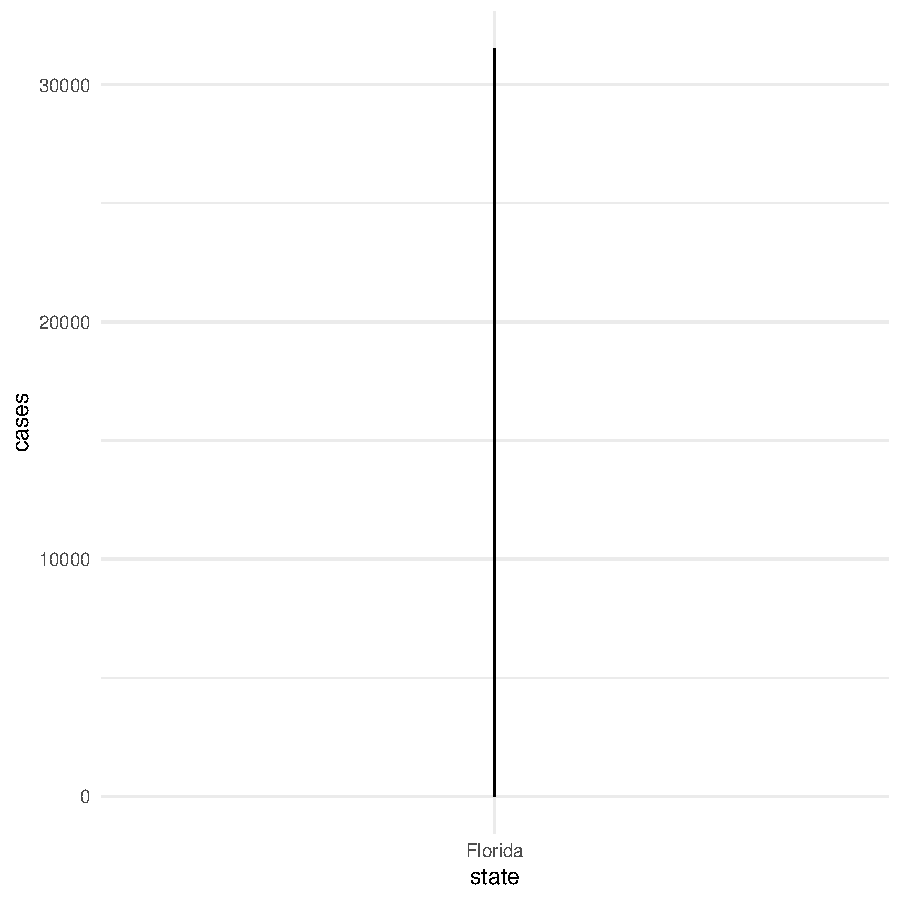
\includegraphics[width=.6\linewidth]{figure/assignment-04-Quintero-Vasquez-Johnatan-Rnwauto-report-6} 

}


\begin{kframe}\begin{alltt}
\hlcom{## Add lines for New York and California to the plot}
\hlkwd{ggplot}\hlstd{(}\hlkwc{data}\hlstd{=florida_df,} \hlkwd{aes}\hlstd{(}\hlkwc{x}\hlstd{=state,} \hlkwc{group}\hlstd{=}\hlnum{1}\hlstd{))} \hlopt{+}
  \hlkwd{geom_line}\hlstd{(}\hlkwd{aes}\hlstd{(}\hlkwc{y} \hlstd{= cases))} \hlopt{+}
  \hlkwd{geom_line}\hlstd{(}\hlkwc{data}\hlstd{=ny_df,} \hlkwd{aes}\hlstd{(}\hlkwc{y} \hlstd{= cases))} \hlopt{+}
  \hlkwd{geom_line}\hlstd{(}\hlkwc{data}\hlstd{=california_df,} \hlkwd{aes}\hlstd{(}\hlkwc{y} \hlstd{= cases))}
\end{alltt}
\end{kframe}

{\centering 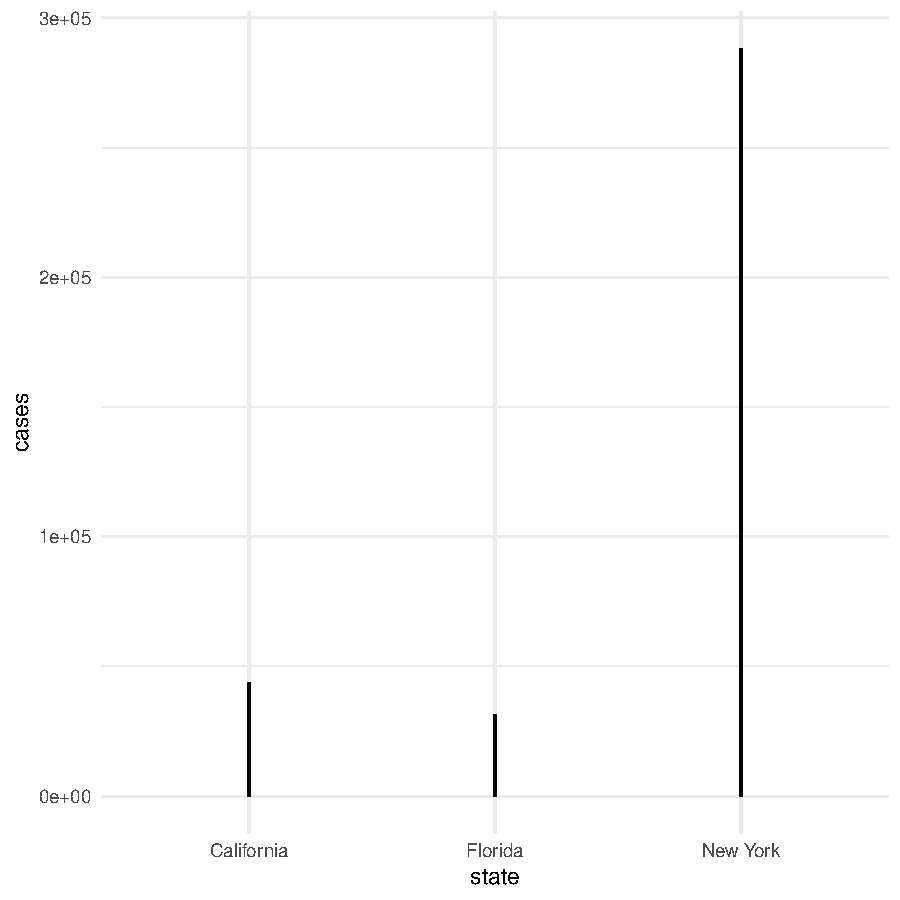
\includegraphics[width=.6\linewidth]{figure/assignment-04-Quintero-Vasquez-Johnatan-Rnwauto-report-7} 

}


\begin{kframe}\begin{alltt}
\hlcom{## Use the colors "darkred", "darkgreen", and "steelblue" for Florida, New York, and California}
\hlkwd{ggplot}\hlstd{(}\hlkwc{data}\hlstd{=florida_df,} \hlkwd{aes}\hlstd{(}\hlkwc{x}\hlstd{=state,} \hlkwc{group}\hlstd{=}\hlnum{1}\hlstd{))} \hlopt{+}
  \hlkwd{geom_line}\hlstd{(}\hlkwd{aes}\hlstd{(}\hlkwc{y} \hlstd{= cases),} \hlkwc{color} \hlstd{=} \hlstr{"darkred"}\hlstd{)} \hlopt{+}
  \hlkwd{geom_line}\hlstd{(}\hlkwc{data}\hlstd{=ny_df,} \hlkwd{aes}\hlstd{(}\hlkwc{y} \hlstd{= cases),} \hlkwc{color} \hlstd{=} \hlstr{"darkgreen"}\hlstd{)} \hlopt{+}
  \hlkwd{geom_line}\hlstd{(}\hlkwc{data}\hlstd{=california_df,} \hlkwd{aes}\hlstd{(}\hlkwc{y} \hlstd{= cases),} \hlkwc{color} \hlstd{=} \hlstr{"steelblue"}\hlstd{)}
\end{alltt}
\end{kframe}

{\centering 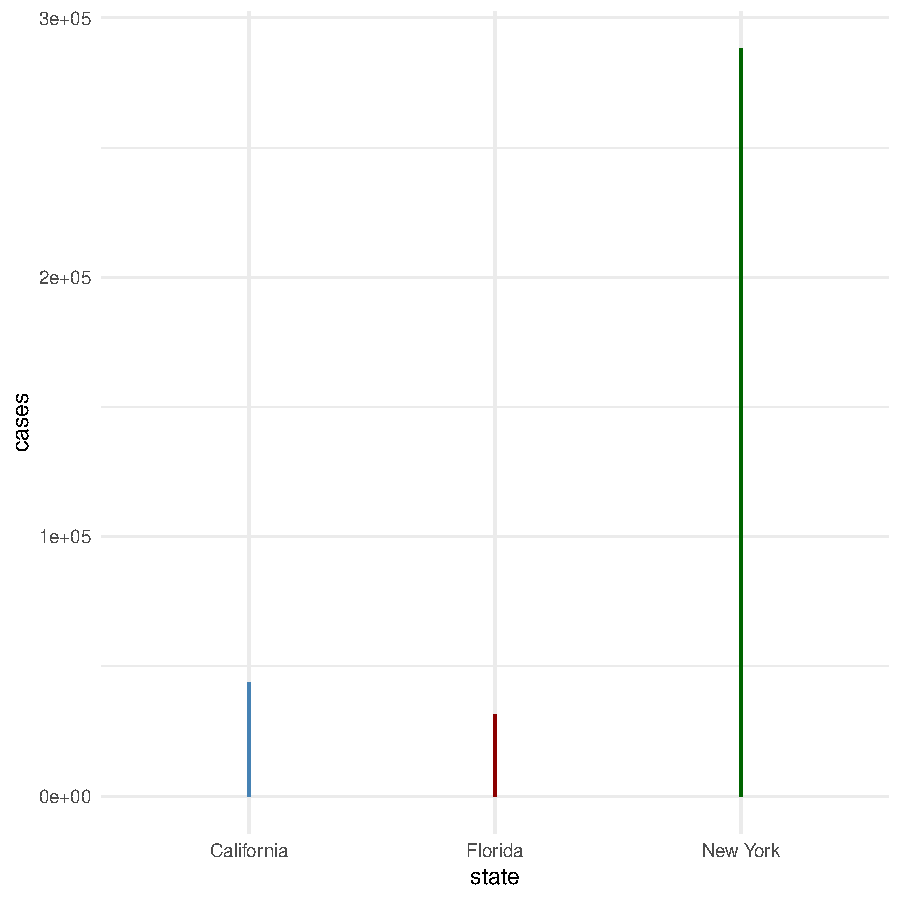
\includegraphics[width=.6\linewidth]{figure/assignment-04-Quintero-Vasquez-Johnatan-Rnwauto-report-8} 

}


\begin{kframe}\begin{alltt}
\hlcom{## Add a legend to the plot using `scale_colour_manual`}
\hlcom{## Add a blank (" ") label to the x-axis and the label "Cases" to the y axis}
\hlkwd{ggplot}\hlstd{(}\hlkwc{data}\hlstd{=florida_df,} \hlkwd{aes}\hlstd{(}\hlkwc{x}\hlstd{=state,} \hlkwc{group}\hlstd{=}\hlnum{1}\hlstd{))} \hlopt{+}
  \hlkwd{geom_line}\hlstd{(}\hlkwd{aes}\hlstd{(}\hlkwc{y} \hlstd{= cases,} \hlkwc{colour} \hlstd{=} \hlstr{"Florida"}\hlstd{))} \hlopt{+}
  \hlkwd{geom_line}\hlstd{(}\hlkwc{data}\hlstd{=ny_df,} \hlkwd{aes}\hlstd{(}\hlkwc{y} \hlstd{= cases,} \hlkwc{colour} \hlstd{=} \hlstr{"New York"}\hlstd{))} \hlopt{+}
  \hlkwd{geom_line}\hlstd{(}\hlkwc{data}\hlstd{=california_df,} \hlkwd{aes}\hlstd{(}\hlkwc{y} \hlstd{= cases,} \hlkwc{colour} \hlstd{=} \hlstr{"California"}\hlstd{))} \hlopt{+}
  \hlkwd{scale_colour_manual}\hlstd{(}\hlstr{"Reported Cases"}\hlstd{,}
                      \hlkwc{breaks} \hlstd{=} \hlkwd{c}\hlstd{(}\hlstr{"Florida"}\hlstd{,} \hlstr{"New York"}\hlstd{,} \hlstr{"California"}\hlstd{),}
                      \hlkwc{values} \hlstd{=} \hlkwd{c}\hlstd{(}\hlstr{"Florida"} \hlstd{=} \hlstr{"darkred"}\hlstd{,} \hlstr{"New York"} \hlstd{=} \hlstr{"darkgreen"}\hlstd{,} \hlstr{"California"} \hlstd{=} \hlstr{"steelblue"}\hlstd{))} \hlopt{+}
    \hlkwd{xlab}\hlstd{(}\hlstr{" "}\hlstd{)} \hlopt{+} \hlkwd{ylab}\hlstd{(}\hlstr{"Cases"}\hlstd{)}
\end{alltt}
\end{kframe}

{\centering 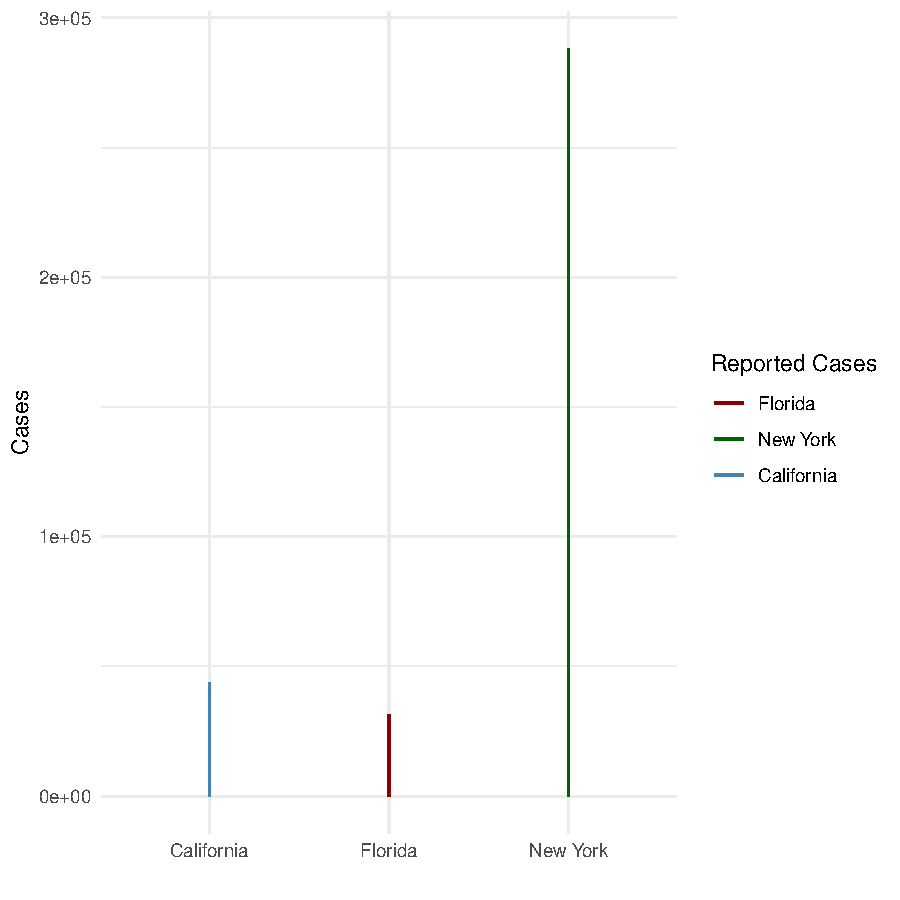
\includegraphics[width=.6\linewidth]{figure/assignment-04-Quintero-Vasquez-Johnatan-Rnwauto-report-9} 

}


\begin{kframe}\begin{alltt}
\hlcom{## Scale the y axis using `scale_y_log10()`}
\hlkwd{ggplot}\hlstd{(}\hlkwc{data}\hlstd{=florida_df,} \hlkwd{aes}\hlstd{(}\hlkwc{x}\hlstd{=state,} \hlkwc{group}\hlstd{=}\hlnum{1}\hlstd{))} \hlopt{+}
  \hlkwd{geom_line}\hlstd{(}\hlkwd{aes}\hlstd{(}\hlkwc{y} \hlstd{= cases,} \hlkwc{colour} \hlstd{=} \hlstr{"Florida"}\hlstd{))} \hlopt{+}
  \hlkwd{geom_line}\hlstd{(}\hlkwc{data}\hlstd{=ny_df,} \hlkwd{aes}\hlstd{(}\hlkwc{y} \hlstd{= cases,} \hlkwc{colour} \hlstd{=} \hlstr{"New York"}\hlstd{))} \hlopt{+}
  \hlkwd{geom_line}\hlstd{(}\hlkwc{data}\hlstd{=california_df,} \hlkwd{aes}\hlstd{(}\hlkwc{y} \hlstd{= cases,} \hlkwc{colour} \hlstd{=} \hlstr{"California"}\hlstd{))} \hlopt{+}
  \hlkwd{scale_colour_manual}\hlstd{(}\hlstr{"Reported Cases"}\hlstd{,}
                      \hlkwc{breaks} \hlstd{=} \hlkwd{c}\hlstd{(}\hlstr{"Florida"}\hlstd{,} \hlstr{"New York"}\hlstd{,} \hlstr{"California"}\hlstd{),}
                      \hlkwc{values} \hlstd{=} \hlkwd{c}\hlstd{(}\hlstr{"Florida"} \hlstd{=} \hlstr{"darkred"}\hlstd{,} \hlstr{"New York"} \hlstd{=} \hlstr{"darkgreen"}\hlstd{,} \hlstr{"California"} \hlstd{=} \hlstr{"steelblue"}\hlstd{))} \hlopt{+}
  \hlkwd{xlab}\hlstd{(}\hlstr{" "}\hlstd{)} \hlopt{+} \hlkwd{ylab}\hlstd{(}\hlstr{"Cases"}\hlstd{)} \hlopt{+} \hlkwd{scale_y_log10}\hlstd{()}
\end{alltt}
\end{kframe}

{\centering 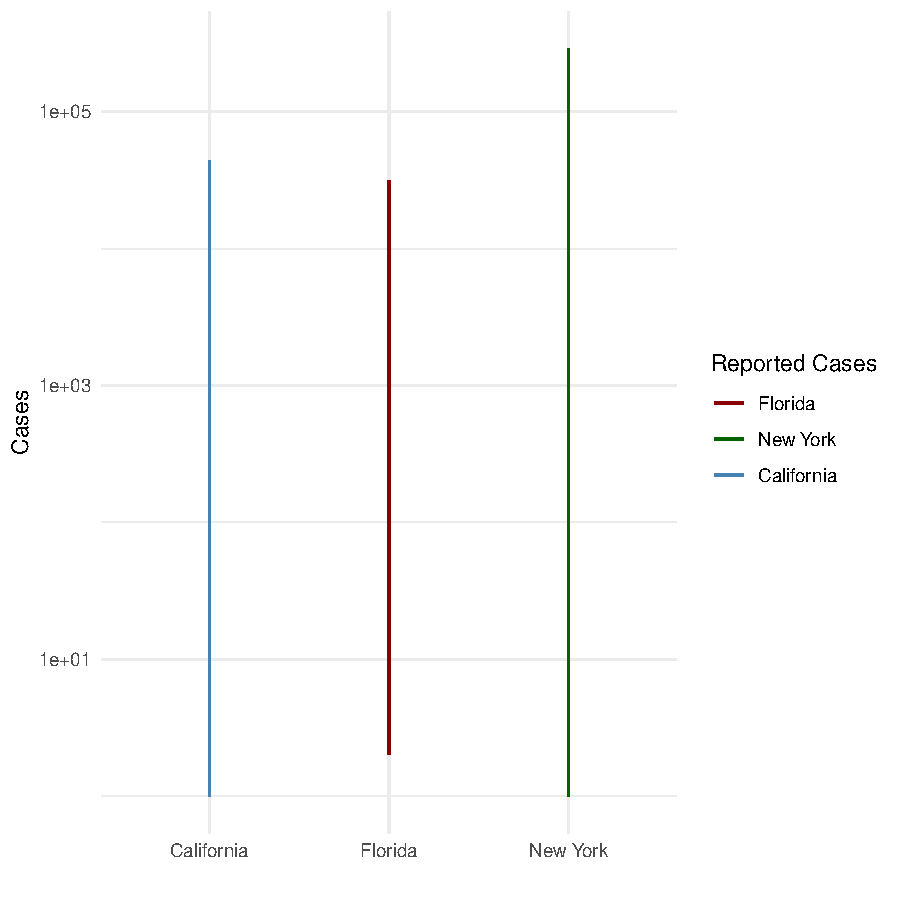
\includegraphics[width=.6\linewidth]{figure/assignment-04-Quintero-Vasquez-Johnatan-Rnwauto-report-10} 

}


\begin{kframe}\begin{alltt}
\hlcom{### knitr::stitch("C:\textbackslash{}\textbackslash{}Users\textbackslash{}\textbackslash{}21428899\textbackslash{}\textbackslash{}OneDrive-Bellevue University\textbackslash{}\textbackslash{}Documents\textbackslash{}\textbackslash{}GitHub\textbackslash{}\textbackslash{}dsc520\textbackslash{}\textbackslash{}assignments\textbackslash{}\textbackslash{}assignment04\textbackslash{}\textbackslash{}assignment_04_Quintero_Vasquez_Johnatan.R")}
\end{alltt}
\end{kframe}
\end{knitrout}

The R session information (including the OS info, R version and all
packages used):

\begin{knitrout}
\definecolor{shadecolor}{rgb}{0.969, 0.969, 0.969}\color{fgcolor}\begin{kframe}
\begin{alltt}
\hlkwd{sessionInfo}\hlstd{()}
\end{alltt}
\begin{verbatim}
## R version 4.3.0 (2023-04-21 ucrt)
## Platform: x86_64-w64-mingw32/x64 (64-bit)
## Running under: Windows 11 x64 (build 22621)
## 
## Matrix products: default
## 
## 
## locale:
## [1] LC_COLLATE=English_United States.utf8  LC_CTYPE=English_United States.utf8   
## [3] LC_MONETARY=English_United States.utf8 LC_NUMERIC=C                          
## [5] LC_TIME=English_United States.utf8    
## 
## time zone: America/New_York
## tzcode source: internal
## 
## attached base packages:
## [1] stats     graphics  grDevices utils     datasets  methods   base     
## 
## other attached packages:
## [1] ggplot2_3.4.2
## 
## loaded via a namespace (and not attached):
##  [1] vctrs_0.6.3      cli_3.6.1        knitr_1.43       rlang_1.1.1      xfun_0.39       
##  [6] highr_0.10       generics_0.1.3   glue_1.6.2       labeling_0.4.2   colorspace_2.1-0
## [11] scales_1.2.1     fansi_1.0.4      grid_4.3.0       munsell_0.5.0    evaluate_0.21   
## [16] tibble_3.2.1     lifecycle_1.0.3  compiler_4.3.0   dplyr_1.1.2      pkgconfig_2.0.3 
## [21] farver_2.1.1     R6_2.5.1         tidyselect_1.2.0 utf8_1.2.3       pillar_1.9.0    
## [26] magrittr_2.0.3   tools_4.3.0      withr_2.5.0      gtable_0.3.3
\end{verbatim}
\begin{alltt}
\hlkwd{Sys.time}\hlstd{()}
\end{alltt}
\begin{verbatim}
## [1] "2023-07-17 04:13:05 EDT"
\end{verbatim}
\end{kframe}
\end{knitrout}


\end{document}
